\chapter{Разработка собственных моделей, адаптация архитектур существующих моделей, улучшения и оптимизация}
\label{sec:Chapter4} \index{Chapter4}

\section{Аппаратные ограничения и вычислительные компромиссы}
\label{subsec:hardware_constraints}

Все эксперименты проводились на рабочей станции с графическим ускорителем NVIDIA RTX 4080 Super (16 ГБ VRAM) и 32 ГБ оперативной памяти. Такая конфигурация налагает жёсткие ограничения на объём обрабатываемых тензоров, размер батча и глубину архитектурных компонентов. При нехватке видеопамяти прямое применение тяжёлых трансформерных блоков, полноразмерного самовнимания либо многомасштабных дискриминаторов исчерпывало память уже на стадии forward-backward pass и дестабилизировало adversarial-обучение.

Приходилось искать баланс между вычислительной сложностью и качеством кросс-модального перевода. Было опробовано несколько конфигураций разной тяжести. Лёгкие варианты с минимумом остаточных блоков, без модулей внимания и с базовой пакетной нормализацией обучались и работали быстро при батче 8--16, однако границы у них размывались, спектр согласовывался плохо, а на сложных ландшафтах заметен был цветовой дрейф. Глубокие многоветвевые конфигурации с CBAM/SelfAttention, частотными ответвлениями и перцептивной регуляризацией восстанавливали структуру точнее и выглядели убедительнее, но требовали снижения батча до 1--4, удлиняли эпоху вдвое-втрое и при неудачной балансировке потерь нередко срывались в осцилляции генератора.

\section{Адаптация существующих моделей}

\subsection{Модификация архитектуры Pix2Pix}
\label{subsec:pix2pix_modifications}

На радиолокационных данных базовая реализация Pix2Pix упирается в несколько системных ограничений. Стандартные свёрточные блоки, транспонированные свёртки и прямые skip-connections порождают шахматные артефакты, размывают границы и расшатывают adversarial-обучение, и тем сильнее, чем меньше батч и выше уровень когерентного шума. Адаптация затронула генератор, дискриминатор и стратегию оптимизации. Усложнение модели не было самоцелью~--- требовалось снять конкретные физические и вычислительные дефекты кросс-модального перевода.

\paragraph{Нормализации}
При \texttt{batch\_size} в пределах 4--8, который только и позволяет лимит видеопамяти, пакетная нормализация теряет устойчивость и искажает градиенты~--- статистика батча в задачах дистанционного зондирования заметно меняется от сцены к сцене. Поэтому \texttt{BatchNorm2d} уступила место \texttt{InstanceNorm2d} в кодировщике и \texttt{GroupNorm} в декодировщике. \texttt{InstanceNorm} аккуратнее сохраняет текстуру и стиль отдельного снимка, а \texttt{GroupNorm} даёт стабильное обучение независимо от размера батча, что важно для воспроизводимости.

\paragraph{Проблема «шахматной доски»}
Транспонированные свёртки склонны порождать периодические паттерны, особенно заметные на однородных участках оптики. Чтобы убрать их, \texttt{ConvTranspose2d} заменён билинейной интерполяцией (\texttt{nn.Upsample}) с последующей обычной свёрткой. Текстуры становятся естественнее, а дискриминатору проще.

\paragraph{Выравнивание признаков}
Переработаны и skip-connections. В исходном U-Net признаки энкодера и декодера конкатенируются напрямую, хотя несут разную семантическую нагрузку и относятся к разным уровням абстракции. Между ними встроены проекционные модули из двойных свёрток с \texttt{GroupNorm} и активацией; они выравнивают распределения признаков перед слиянием и сокращают информационный разрыв между масштабами. Линейные объекты при этом получаются чётче, а «швы» на границах рецептивных полей уменьшаются.

\paragraph{Пространственное и канальное внимание}
В bottleneck стандартные остаточные блоки заменены на \texttt{UNetResidualBlock} с CBAM и \texttt{SelfAttention}. CBAM взвешивает каналы и пространственные регионы: зашумлённые спеклом зоны подавляются, структурно значимые фрагменты усиливаются. \texttt{SelfAttention} улавливает дальние зависимости в латентном пространстве, поэтому модель согласует удалённые части сцены и не разрывает протяжённые линейные объекты.

\paragraph{Инициализация и вычислительные оптимизации}
Стандартный \texttt{Tanh} легко насыщается, а отсюда цветовой дрейф и «плоские» регионы с нулевыми градиентами. Выходной блок поэтому переработан в трёхступенчатую структуру, а веса финального слоя инициализированы со стандартным отклонением \texttt{std=0.005}: уменьшенная дисперсия и промежуточные нелинейности удерживают оптимизацию вблизи нуля, сглаживают цветовое распределение и ускоряют сходимость на поздних эпохах. Предусмотрена и подача вместе с SAR-изображением вспомогательной информации, например семантической карты, которая снижает некорректность задачи раскраски.

Изменения коснулись и дискриминатора~--- ради устойчивости minimax-игры. На все свёрточные слои наложена спектральная нормализация: она ограничивает константу Липшица, гасит взрыв градиентов и заметно сглаживает кривые потерь. \texttt{BatchNorm} заменён на \texttt{InstanceNorm}, что снимает зависимость от статистики батча и точнее оценивает локальные текстуры при сезонных и ландшафтных сдвигах. На втором уровне даунсэмплинга добавлен \texttt{SelfAttention}, и теперь дискриминатор судит не только об отдельных патчах, но и о глобальной компоновке сцены. Внимание помогает ловить структурные несоответствия, мимо которых чистый PatchGAN обычно проходит: выдуманные объекты и неестественные границы между классами.

Функция потерь складывается из состязательной LSGAN~\eqref{eq:lsgan_loss} (вес 1.5) и пиксельной $L_1$~\eqref{eq:l1_l2} (вес 165). По сравнению с классическим BCE LSGAN даёт более плавные градиенты и гасит осцилляции~--- на зашумлённых SAR-входах это особенно ценно. Высокий относительный вес $L_1$ удерживает выход привязанным к эталону по структуре и подавляет цветовой дрейф. Перцептивные и feature-matching ограничения в базовой реализации не используются: они появляются позднее, в собственных моделях семейства LLW-Former (подраздел~\ref{subsec:llwformer}).

\begin{figure}[!ht]
    \centering
    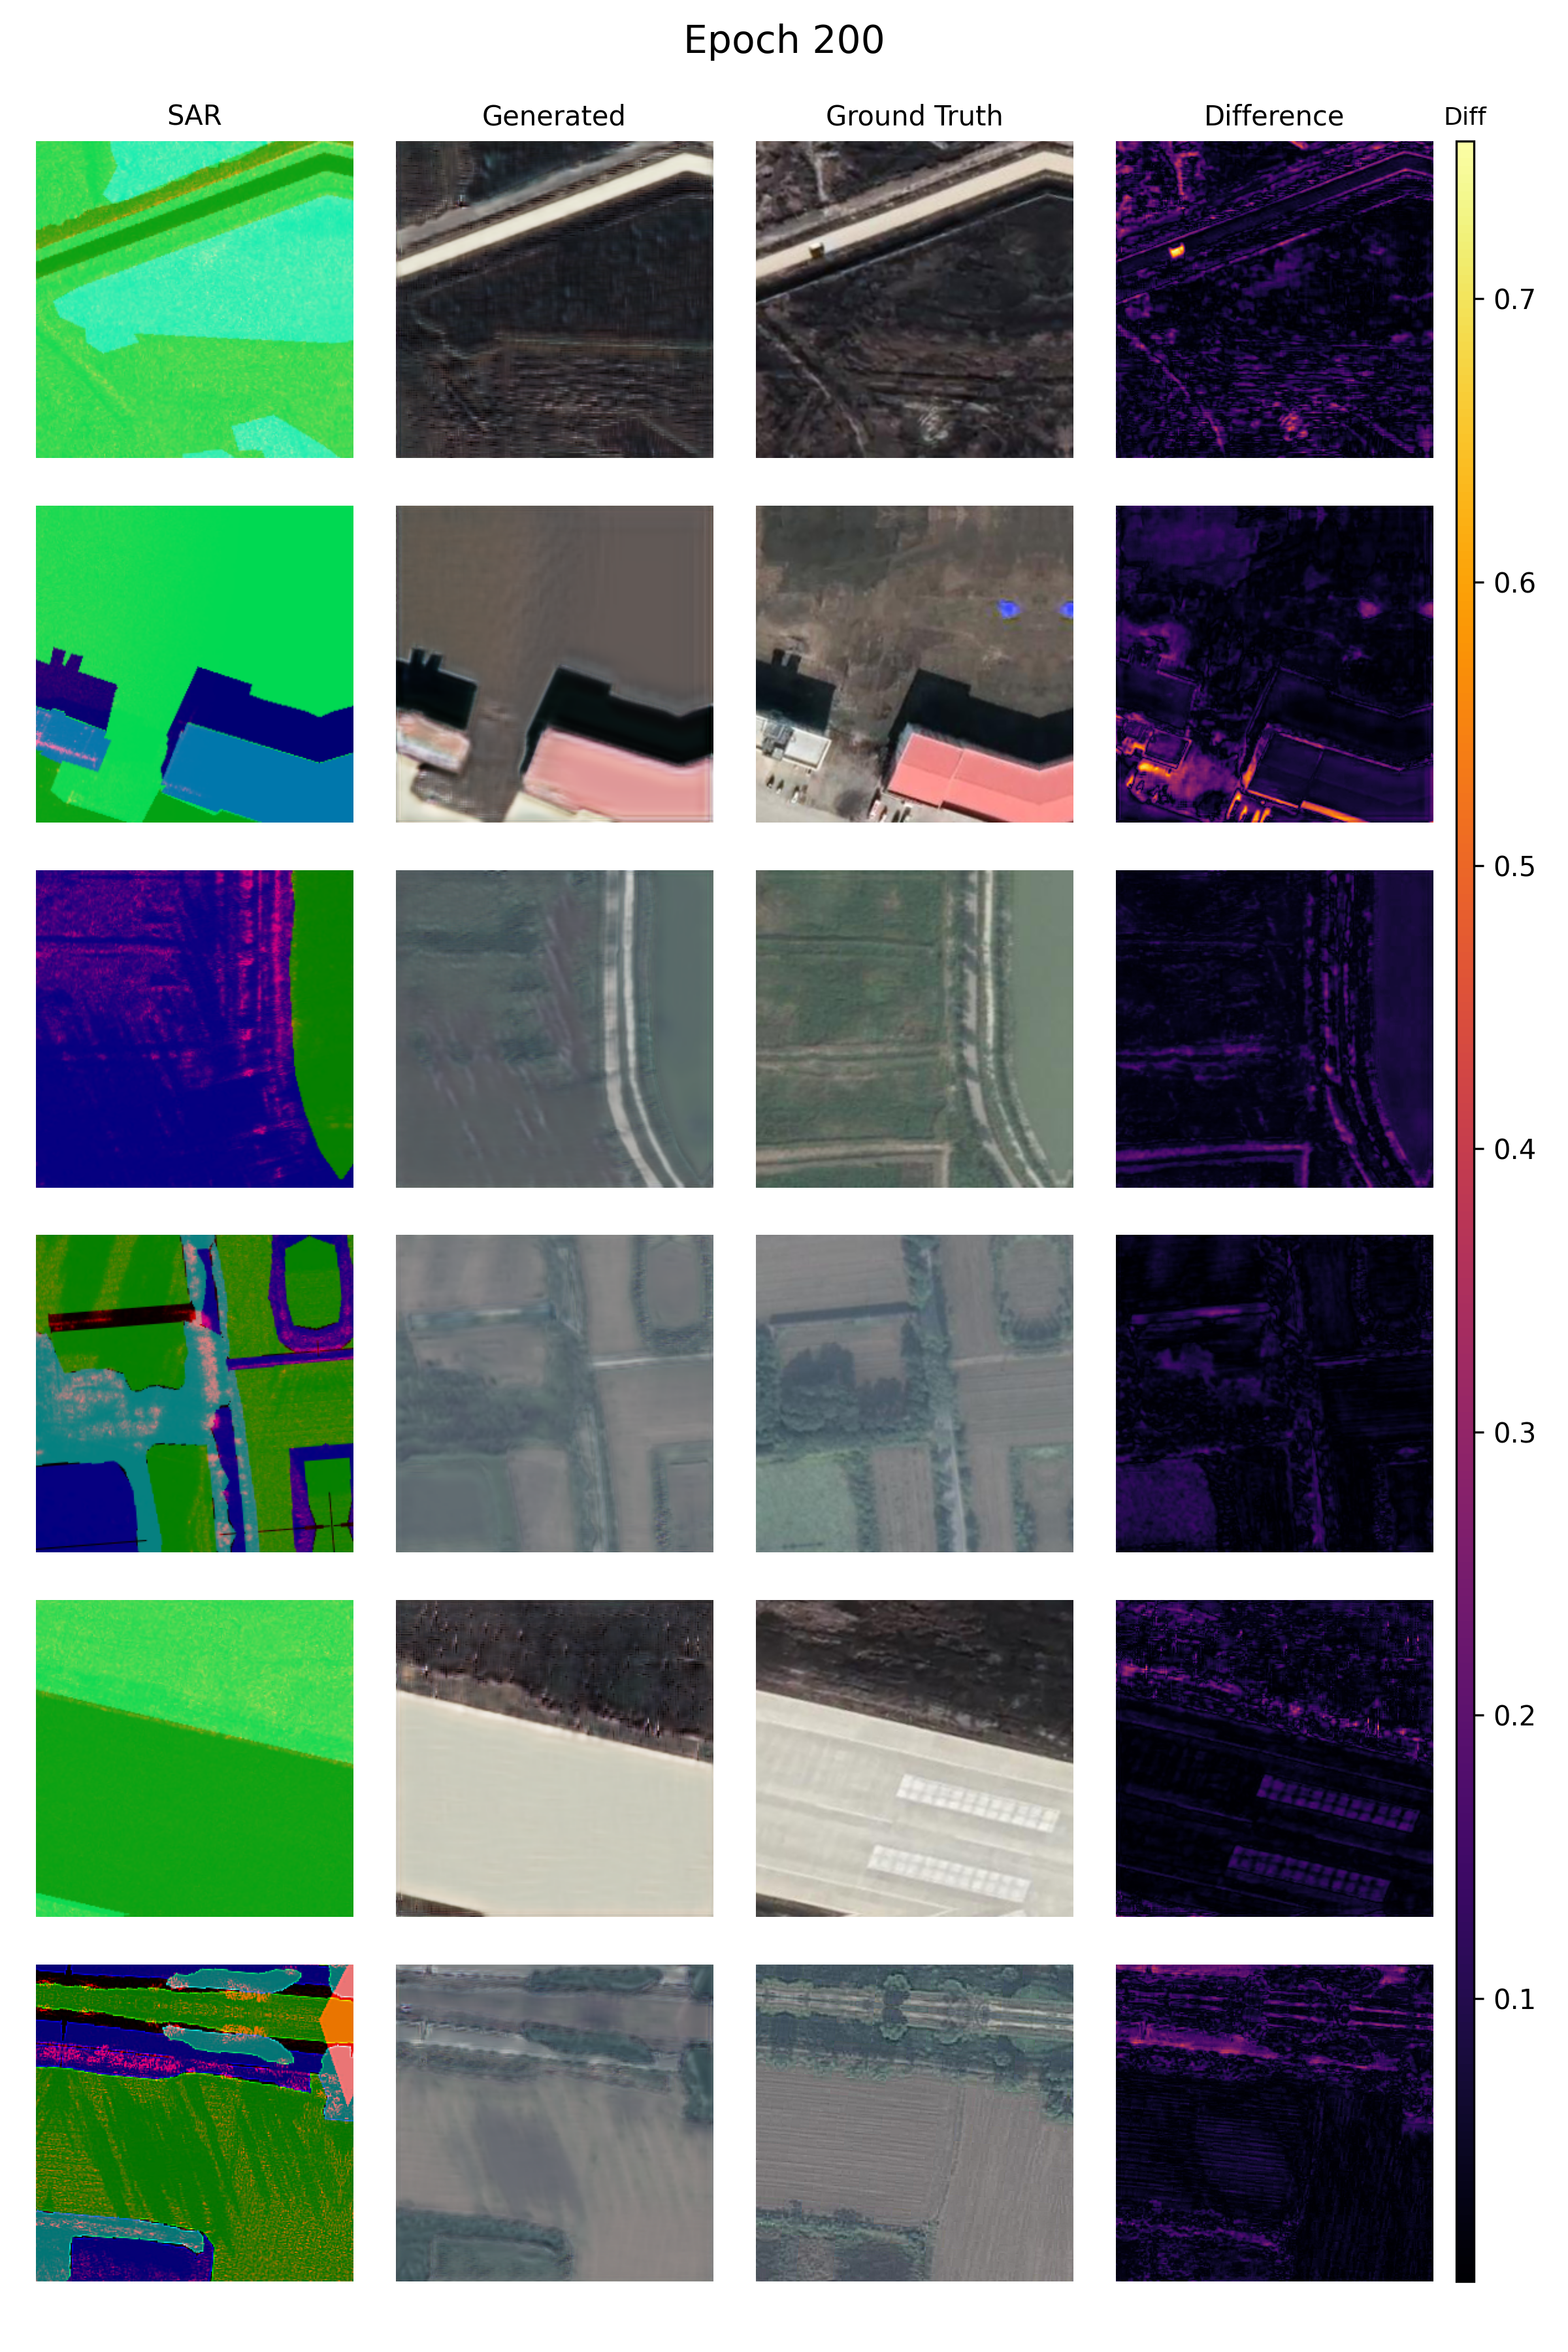
\includegraphics[width=0.8\linewidth]{images/pix2pix/output/pix2pix_labeled.png}
    \caption{Результат обучения модифицированной модели Pix2Pix на семантически размеченном датасете на протяжении 200 эпох.}
    \label{fig:pix2pix_sar2opt_labeled_200ep}
\end{figure}

На рисунке~\ref{fig:pix2pix_sar2opt_labeled_200ep} видно, что Pix2Pix восстанавливает общую структуру сцены и основные цветовые регионы, разделяя зелень растительности, водную синеву и серую урбанизированную застройку. И всё же даже после CBAM, адаптивных skip-connections и спектральной нормализации модель размывает границы классов, локально дрейфует по цвету в зонах сложного рельефа и плохо связывает протяжённые линейные объекты~--- например, оставляет русло реки разорванным. Природа этих артефактов архитектурная. Локальное рецептивное поле свёрток и отсутствие явного моделирования non-local зависимостей не дают точно согласовать радиолокационную интенсивность с оптическим цветовым пространством. Отсюда и переход к специализированным моделям~--- к собственной архитектуре, которая явно учитывает глобальный контекст, дальние пространственные связи и кросс-модальное выравнивание признаков.


\subsection{Архитектурные модификации в реализации модели, вдохновлённой CFRWD}
\label{subsec:cfrwd_modifications}

При адаптации архитектуры, концептуально опирающейся на CFRWD-GAN~\cite{wei2023cfrwd}, внесён ряд целевых изменений. Их общая задача~--- удержать обучение устойчивым при ограниченных ресурсах, сохранив структурную целостность сцены и не наплодив артефактов генерации. Ключевые отличия реализации от оригинальной публикации перечислены далее.

\paragraph{Пространственно-адаптивное слияние ветвей}
В оригинальной работе~\cite{wei2023cfrwd} выходы CFR- и WD-ветвей объединяются через скалярный обучаемый коэффициент $\alpha$:
\begin{equation}
    y = \alpha \cdot y_{\text{CFR}} + (1 - \alpha) \cdot y_{\text{WD}}, \quad \alpha \in [0, 1].
\end{equation}
Скаляр $\alpha$ не учитывает пространственную неоднородность сцен: где-то доминирует семантика (CFR), где-то~--- высокочастотные детали (WD).

В предлагаемой реализации введён механизм \textit{AdaptiveFusion}, формирующий карту весов на уровне признаков:
\begin{equation}
    W = \operatorname{softmax}\bigl( \operatorname{Conv}_{1\times1}(\operatorname{cat}(f_{\text{CFR}}, f_{\text{WD}})) \bigr), \quad
    f_{\text{fused}} = W_0 \odot f_{\text{CFR}} + W_1 \odot f_{\text{WD}},
\end{equation}
где $W \in \mathbb{R}^{B \times 2 \times H \times W}$, $\odot$~--- поэлементное умножение. Вклад ветвей распределяется теперь по локальному контексту: на границах объектов включается частотная ветвь, в однородных областях~--- семантическая. Градиент функции потерь поступает в обе ветви равномерно, и ни одна из них не затухает по ходу обучения.

\paragraph{Независимые потоки в частотной ветви}
В оригинальной статье~\cite{wei2023cfrwd} высокочастотные группы вейвлет-коэффициентов ($g_2 = [LH_2, HL_2, HH_2]$, $g_3 = [LH_1, HL_1, HH_1]$) суммируются до обработки в HFCF; текстурные паттерны разных масштабов при этом перемешиваются, а фильтрация теряет в эффективности. В предлагаемой реализации каждая группа идёт по \textit{отдельному потоку} с собственным модулем предобработки, CBAM и остаточными блоками:
\begin{itemize}
    \item \textbf{Low-freq stream} ($LL_2$): структурный контекст сцены, обрабатывается через \texttt{WDResBlock} (bottleneck-архитектура);
    \item \textbf{Mid-freq stream} ($[LH_2, HL_2, HH_2]$): детали среднего масштаба, обрабатываются через 6 \texttt{WDResBlock} (чередование проекционных и стандартных остаточных блоков);
    \item \textbf{High-freq stream} ($[LH_1, HL_1, HH_1]$): тонкие границы, обрабатываются через 2 \texttt{RedBlock} (базовый остаточный блок).
\end{itemize}
Объединяются потоки лишь в конце, свёрткой $1 \times 1$. Раздельная обработка даёт подобрать глубину и ёмкость под каждый частотный диапазон и подавить спекл-шум без потери истинных границ.

\paragraph{Пространственно-канальное внимание в частотной ветви}
В каждый поток частотной ветви встроен CBAM~\cite{woo2018cbam}~--- он последовательно применяет канальное и пространственное внимание и за счёт этого повышает селективность фильтрации:
\begin{equation}
    x' = x \cdot \sigma\bigl( \operatorname{MLP}(\operatorname{AvgPool}(x)) + \operatorname{MLP}(\operatorname{MaxPool}(x)) \bigr), \quad
    x'' = x' \cdot \sigma\bigl( \operatorname{Conv}_{7\times7}(\operatorname{cat}(\overline{x'}, \widehat{x'})) \bigr),
\end{equation}
где $\overline{x'}$, $\widehat{x'}$~--- среднее и максимум по каналам. В задаче SAR$\to$Optical CBAM гасит спектрально незначимые зоны, зашумлённые спеклом, и усиливает коэффициенты реальных структур~--- например, чёткой границы между полем и лесополосой.

\paragraph{Стабилизация дискриминатора и стратегии оптимизации}
Для повышения устойчивости \textit{adversarial}-обучения внесены следующие изменения:
\begin{itemize}
    \item спектральная нормализация на всех свёрточных слоях дискриминатора ограничивает константу Липшица и не даёт градиентам и потерям сорваться в осцилляции;
    \item двухмасштабный анализ: дискриминатор оценивает пары на исходном разрешении и после билинейного даунсэмплинга, что улучшает согласованность глобальной структуры и локальных текстур;
    \item целевая функция многокомпонентна (состязательная LSGAN, Feature Matching с весом~10 и вспомогательная частотная) и комбинируется фиксированными весами, подобранными эмпирически.
\end{itemize}

\paragraph{Инициализация и вычислительные оптимизации}
Для ускорения сходимости и повышения стабильности:
\begin{itemize}
    \item веса финального свёрточного слоя инициализированы методом Ксавье с поправкой под нелинейность \texttt{Tanh} (\texttt{xavier\_normal} с соответствующим \texttt{gain}), что снижает риск насыщения и стабилизирует градиенты на поздних эпохах;
    \item \texttt{Upsample} с билинейной интерполяцией заменяет \texttt{ConvTranspose2d} и убирает шахматные артефакты;
    \item \texttt{InstanceNorm} во всех блоках снимает зависимость от статистики батча и держит обучение стабильным при малом размере батча ($\texttt{batch\_size} = 1\text{--}4$).
\end{itemize}

\paragraph{Визуализация результатов}

Официального исходного кода и подробных спецификаций обучения публикация~\cite{wei2023cfrwd} не приводит, поэтому точно воспроизвести оригинальную конфигурацию CFRWD-GAN и сопоставить её с адаптацией один к одному не удалось. Приведённые визуализации показывают качество трансляции модифицированной архитектуры на валидационной выборке и эффект от внедрённых инженерных решений. Дополнительные примеры вынесены в приложение (рис.~\ref{fig:appendix_cfrwd_val_figures_1-3} и рис.~\ref{fig:appendix_cfrwd_val_figures_4-7}).

\begin{figure}[!ht]
    \centering
    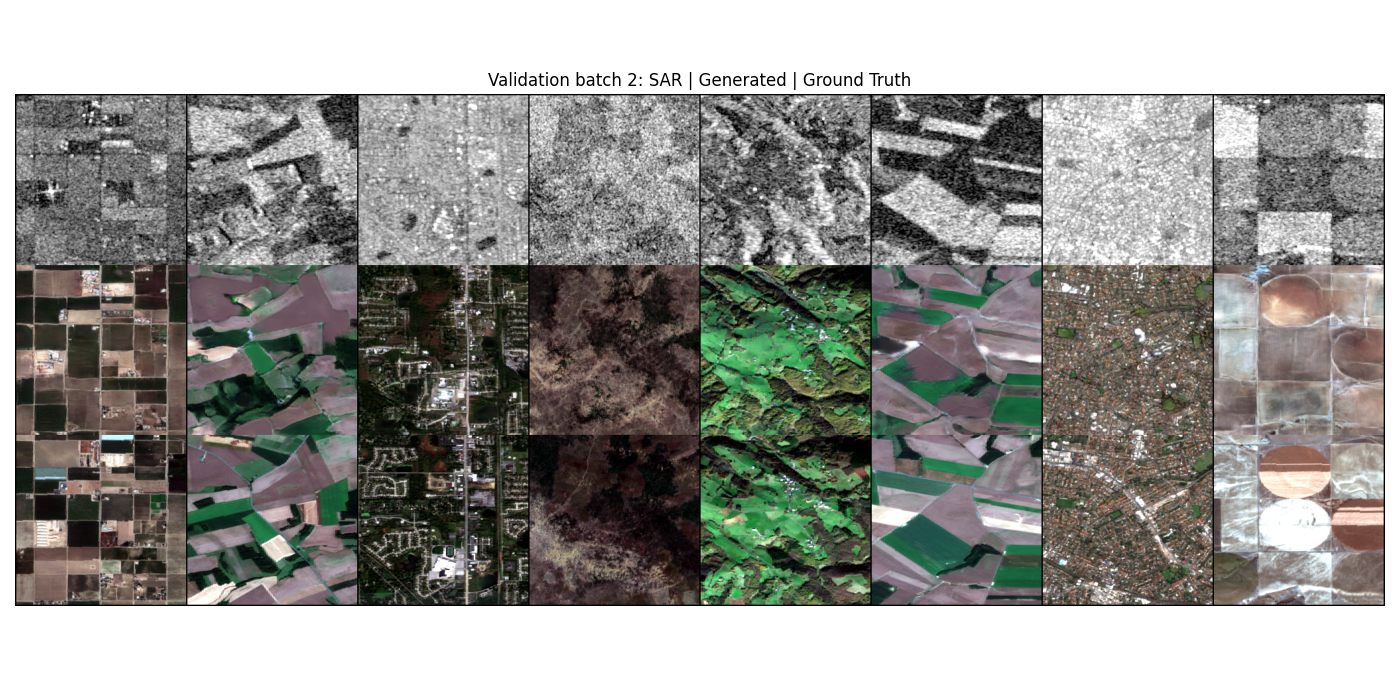
\includegraphics[width=0.95\linewidth]{images/cfrwd/output/val/Figure_2.png}
    \caption{Примеры трансляции SAR-изображений в урбанизированной и пригородной зонах. Строки сверху вниз: (а) входное радиолокационное изображение; (б) результат генерации модифицированной модели; (в) целевое оптическое изображение (ground truth).}
    \label{fig:cfrwd_val_fig_2}
\end{figure}

\begin{figure}[!ht]
    \centering
    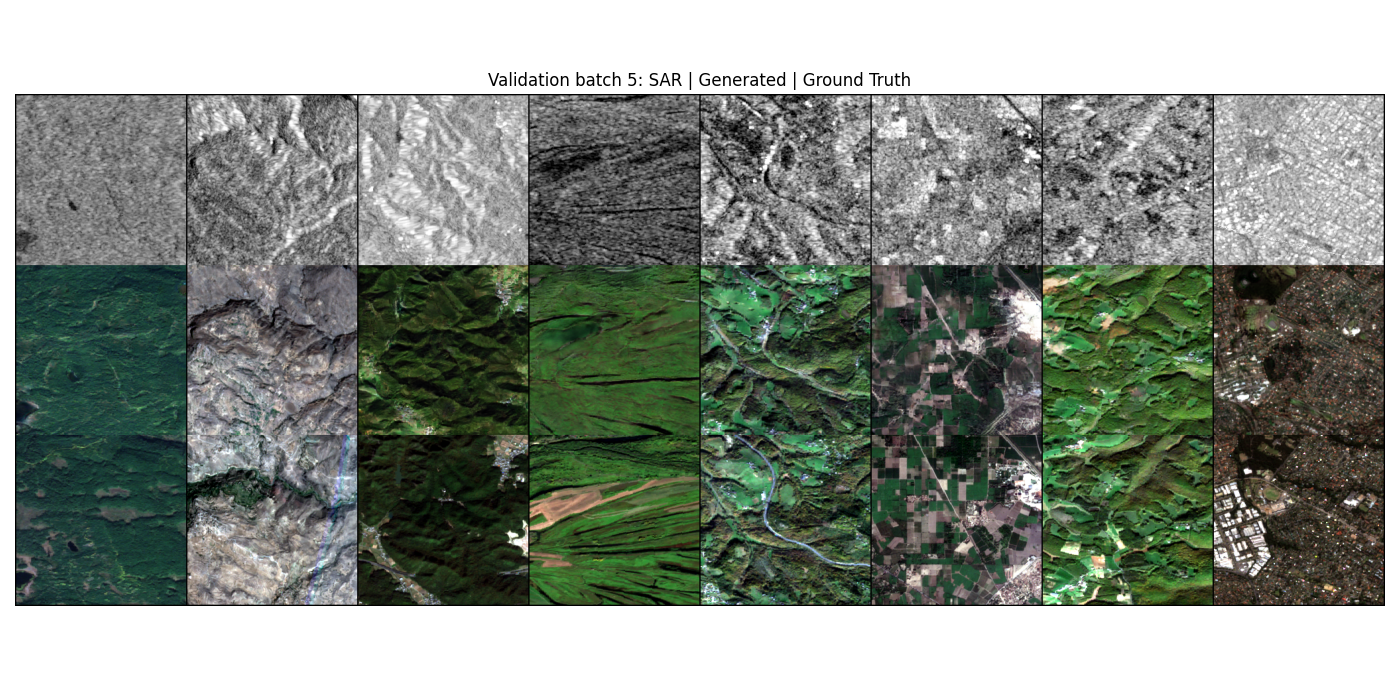
\includegraphics[width=0.95\linewidth]{images/cfrwd/output/val/Figure_5.png}
    \caption{Примеры трансляции в сельскохозяйственных и природных зонах. Обозначения аналогичны рис.~\ref{fig:cfrwd_val_fig_2}.}
    \label{fig:cfrwd_val_fig_5}
\end{figure}

Работа модифицированного генератора во многом сводится к взаимодействию двух ветвей обработки. Рисунок~\ref{fig:epoch_270} детально показывает отдельные компоненты архитектуры на этапе обучения (эпоха 270).

\begin{figure}[!ht]
    \centering
    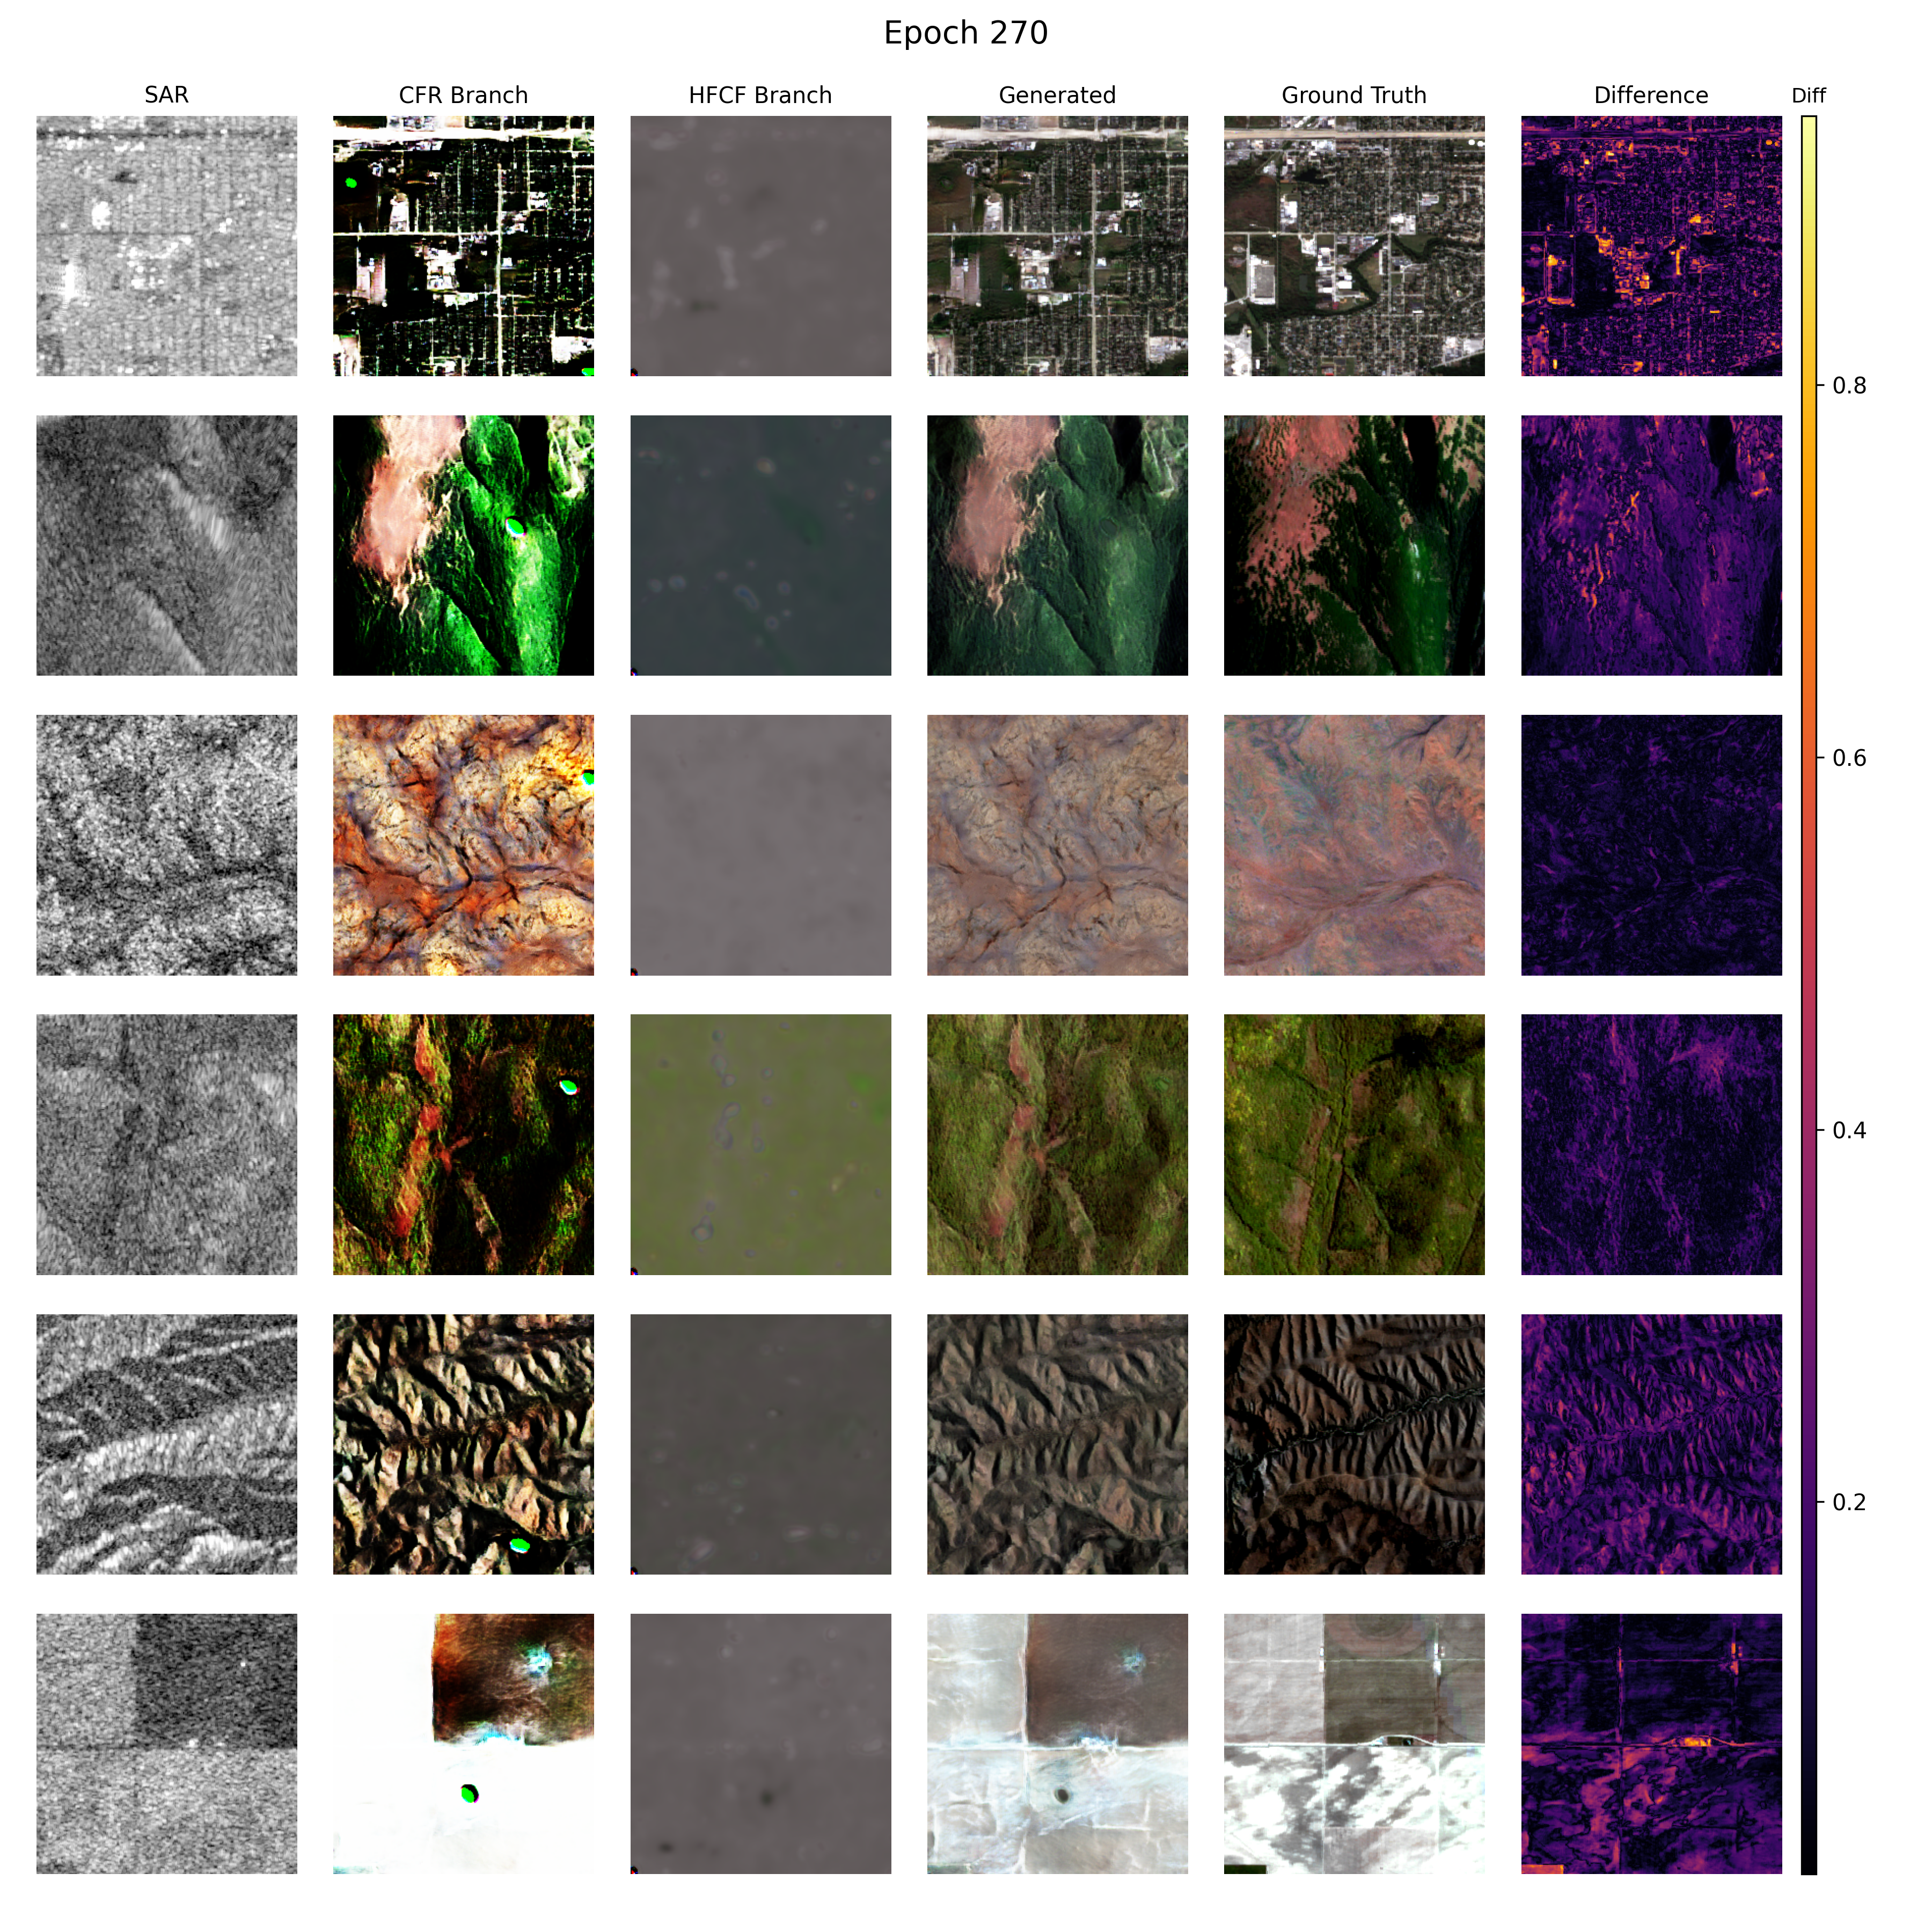
\includegraphics[width=0.98\linewidth]{images/cfrwd/output/train/epoch_270.png}
    \caption{Детальная визуализация работы ветвей генератора. Столбцы слева направо: (а) входное SAR-изображение; (б) выход CFR-ветви (семантический каркас); (в) выход HFCF-ветви (высокочастотные детали); (г) итоговое сгенерированное изображение (после \textit{AdaptiveFusion}); (д) целевое изображение (ground truth); (е) карта разностей (Difference) с цветовой шкалой ошибки.}
    \label{fig:epoch_270}
\end{figure}

На рисунке~\ref{fig:epoch_270} хорошо видно функциональное разделение ветвей и работу механизма \textit{AdaptiveFusion}.

\begin{itemize}
    \item \textbf{CFR Branch (Семантический каркас):} ветвь CFR восстанавливает структуру сцены и глобальное цветовое распределение. На рисунке она уверенно разводит основные классы покрытия~--- застройку, открытый грунт и растительность. Местами, однако (например, в первой строке урбанизированной застройки), проступают локальные артефакты цветового дрейфа~--- яркие неестественные пятна там, где спекл-шум принят за значимую структуру.
    \item \textbf{HFCF Branch (Высокочастотные детали):} ветвь HFCF на вейвлет-разложении извлекает граничные структуры и текстуры. Её выход~--- карта тонких деталей, дополняющая семантическую базу.
    \item \textbf{Adaptive Fusion (Результат):} адаптивное слияние сводит вместе сильные стороны обеих ветвей. В итоговом изображении (столбец \textit{Generated}) артефакты CFR-ветви подавлены, а текстурная чёткость поднята данными HFCF.
    \item \textbf{Карта разностей (Difference):} последний столбец показывает распределение ошибки. На большей части кадра преобладают тёмные тона (фиолетовый/синий), то есть расхождение с эталоном мало. Всплески яркости (жёлтый/оранжевый) сосредоточены в сложных граничных зонах и областях с высокой вариативностью текстуры, где неопределённость задачи максимальна.
\end{itemize}

Визуальный анализ подтверждает, что разделение ответственности между семантической (CFR) и текстурной (HFCF) ветвями под управлением адаптивного слияния компенсирует слабости каждого компонента и поднимает итоговое качество трансляции.

\subsection{Методологический итог}
\label{subsec:inspired_models_methodological_summary}

Все рассмотренные модификации~--- от адаптации базовых условных GAN-каркасов до специализированной многоветвевой архитектуры на принципах CFRWD-GAN~\cite{wei2023cfrwd}~--- подчинены единой логике: неинформативные на радиолокационных данных операции заменяются доменно-специфичными модулями, а само adversarial-обучение стабилизируется под ограниченные ресурсы. Описанные выше решения для генератора, механизмов внимания, нормализации, дискриминатора и функции потерь служат именно этой цели~--- снять потерю семантики при пространственном рассуждении, чувствительность к когерентному шуму и неустойчивость сходимости. Совокупно они превращают универсальные каркасы трансляции в специализированные инструменты, устойчивые к физической специфике SAR-изображений, что согласуется с качественным анализом и картами разностей из предыдущих подразделов. Количественная проверка этих улучшений и сравнение с альтернативными подходами вынесены в следующий раздел.


\section{Разработка собственных моделей}

\subsection{Легковесная иерархическая архитектура с контекстным вниманием}
\label{subsec:lightweight_hierarchical_model}

При ограниченных ресурсах и требовании к скорости инференса разработана легковесная иерархическая архитектура, балансирующая структурную точность трансляции и вычислительную эффективность. Экстрактором признаков служит предобученный на ImageNet каркас ConvNeXtV2. Статистика естественных изображений и SAR-изображений различается принципиально: ImageNet~--- трёхканальные данные с выраженными спектральными градиентами и богатой текстурой, SAR-изображение~--- одноканальная интенсивность обратного рассеяния, отягощённая когерентным шумом и геометрическими искажениями. Если подать доменно-специфичные признаки без адаптации, латентные пространства катастрофически рассогласуются. Разрыв закрывает адаптивный проекционный модуль \texttt{ChannelAdapter}: он переводит одноканальный SAR-вход в трёхканальное представление под требования входного ствола ConvNeXtV2 и попутно нормирует радиометрию.

Латентное представление с глубинного уровня энкодера ($8\times8$ пространственных токенов) проходит через модуль глобального самовнимания \texttt{BottleneckAttention} на базе \texttt{nn.TransformerEncoder}. Внимание стоит только в bottleneck-зоне; так оно улавливает дальние пространственные зависимости и собирает единый семантический контекст сцены без квадратичного роста сложности, характерного для полноразмерного self-attention. Разрешение восстанавливает каскад модулей \texttt{ConvUpsampleBlock}; каждый сочетает билинейную интерполяцию, конкатенацию со skip-признаками своего уровня энкодера и двухступенчатую свёртку с групповой нормализацией (\texttt{GroupNorm}) и активацией GELU. \texttt{GroupNorm} удерживает градиентный поток устойчивым при малых батчах и сглаживает статистические флуктуации в выборках дистанционного зондирования. Остаточные связи внутри декодерных блоков сохраняют высокочастотные градиенты и ускоряют сходимость. Финальная проекция в трёхканальное оптическое пространство выполняется свёрточным блоком $7\times7$ с нелинейностью \texttt{Tanh}.

Дискриминатор~--- двухмасштабный PatchGAN со спектральной нормализацией всех свёрточных слоёв, что ограничивает \textit{Lipschitz}-константу критика и стабилизирует минимакс-игру. Целевая функция объединяет состязательную потерю (LSGAN) с плавными градиентами на поздних эпохах и высокоразмерную \textit{Feature Matching Loss} по промежуточным картам признаков дискриминатора. Спектральную согласованность дополнительно контролирует частотная потеря (\textit{FFTLoss}) на логарифмических амплитудных спектрах, а структуру стабилизирует перцептивная потеря на признаках замороженного экстрактора. Баланс компонент задан фиксированными эмпирическими весами: состязательная~--- 1.0, Feature Matching~--- 5.0, частотная~--- 1.0, перцептивная~--- 0.1.

\paragraph{Результаты обучения: визуальный анализ}

\begin{figure}[!ht]
    \centering
    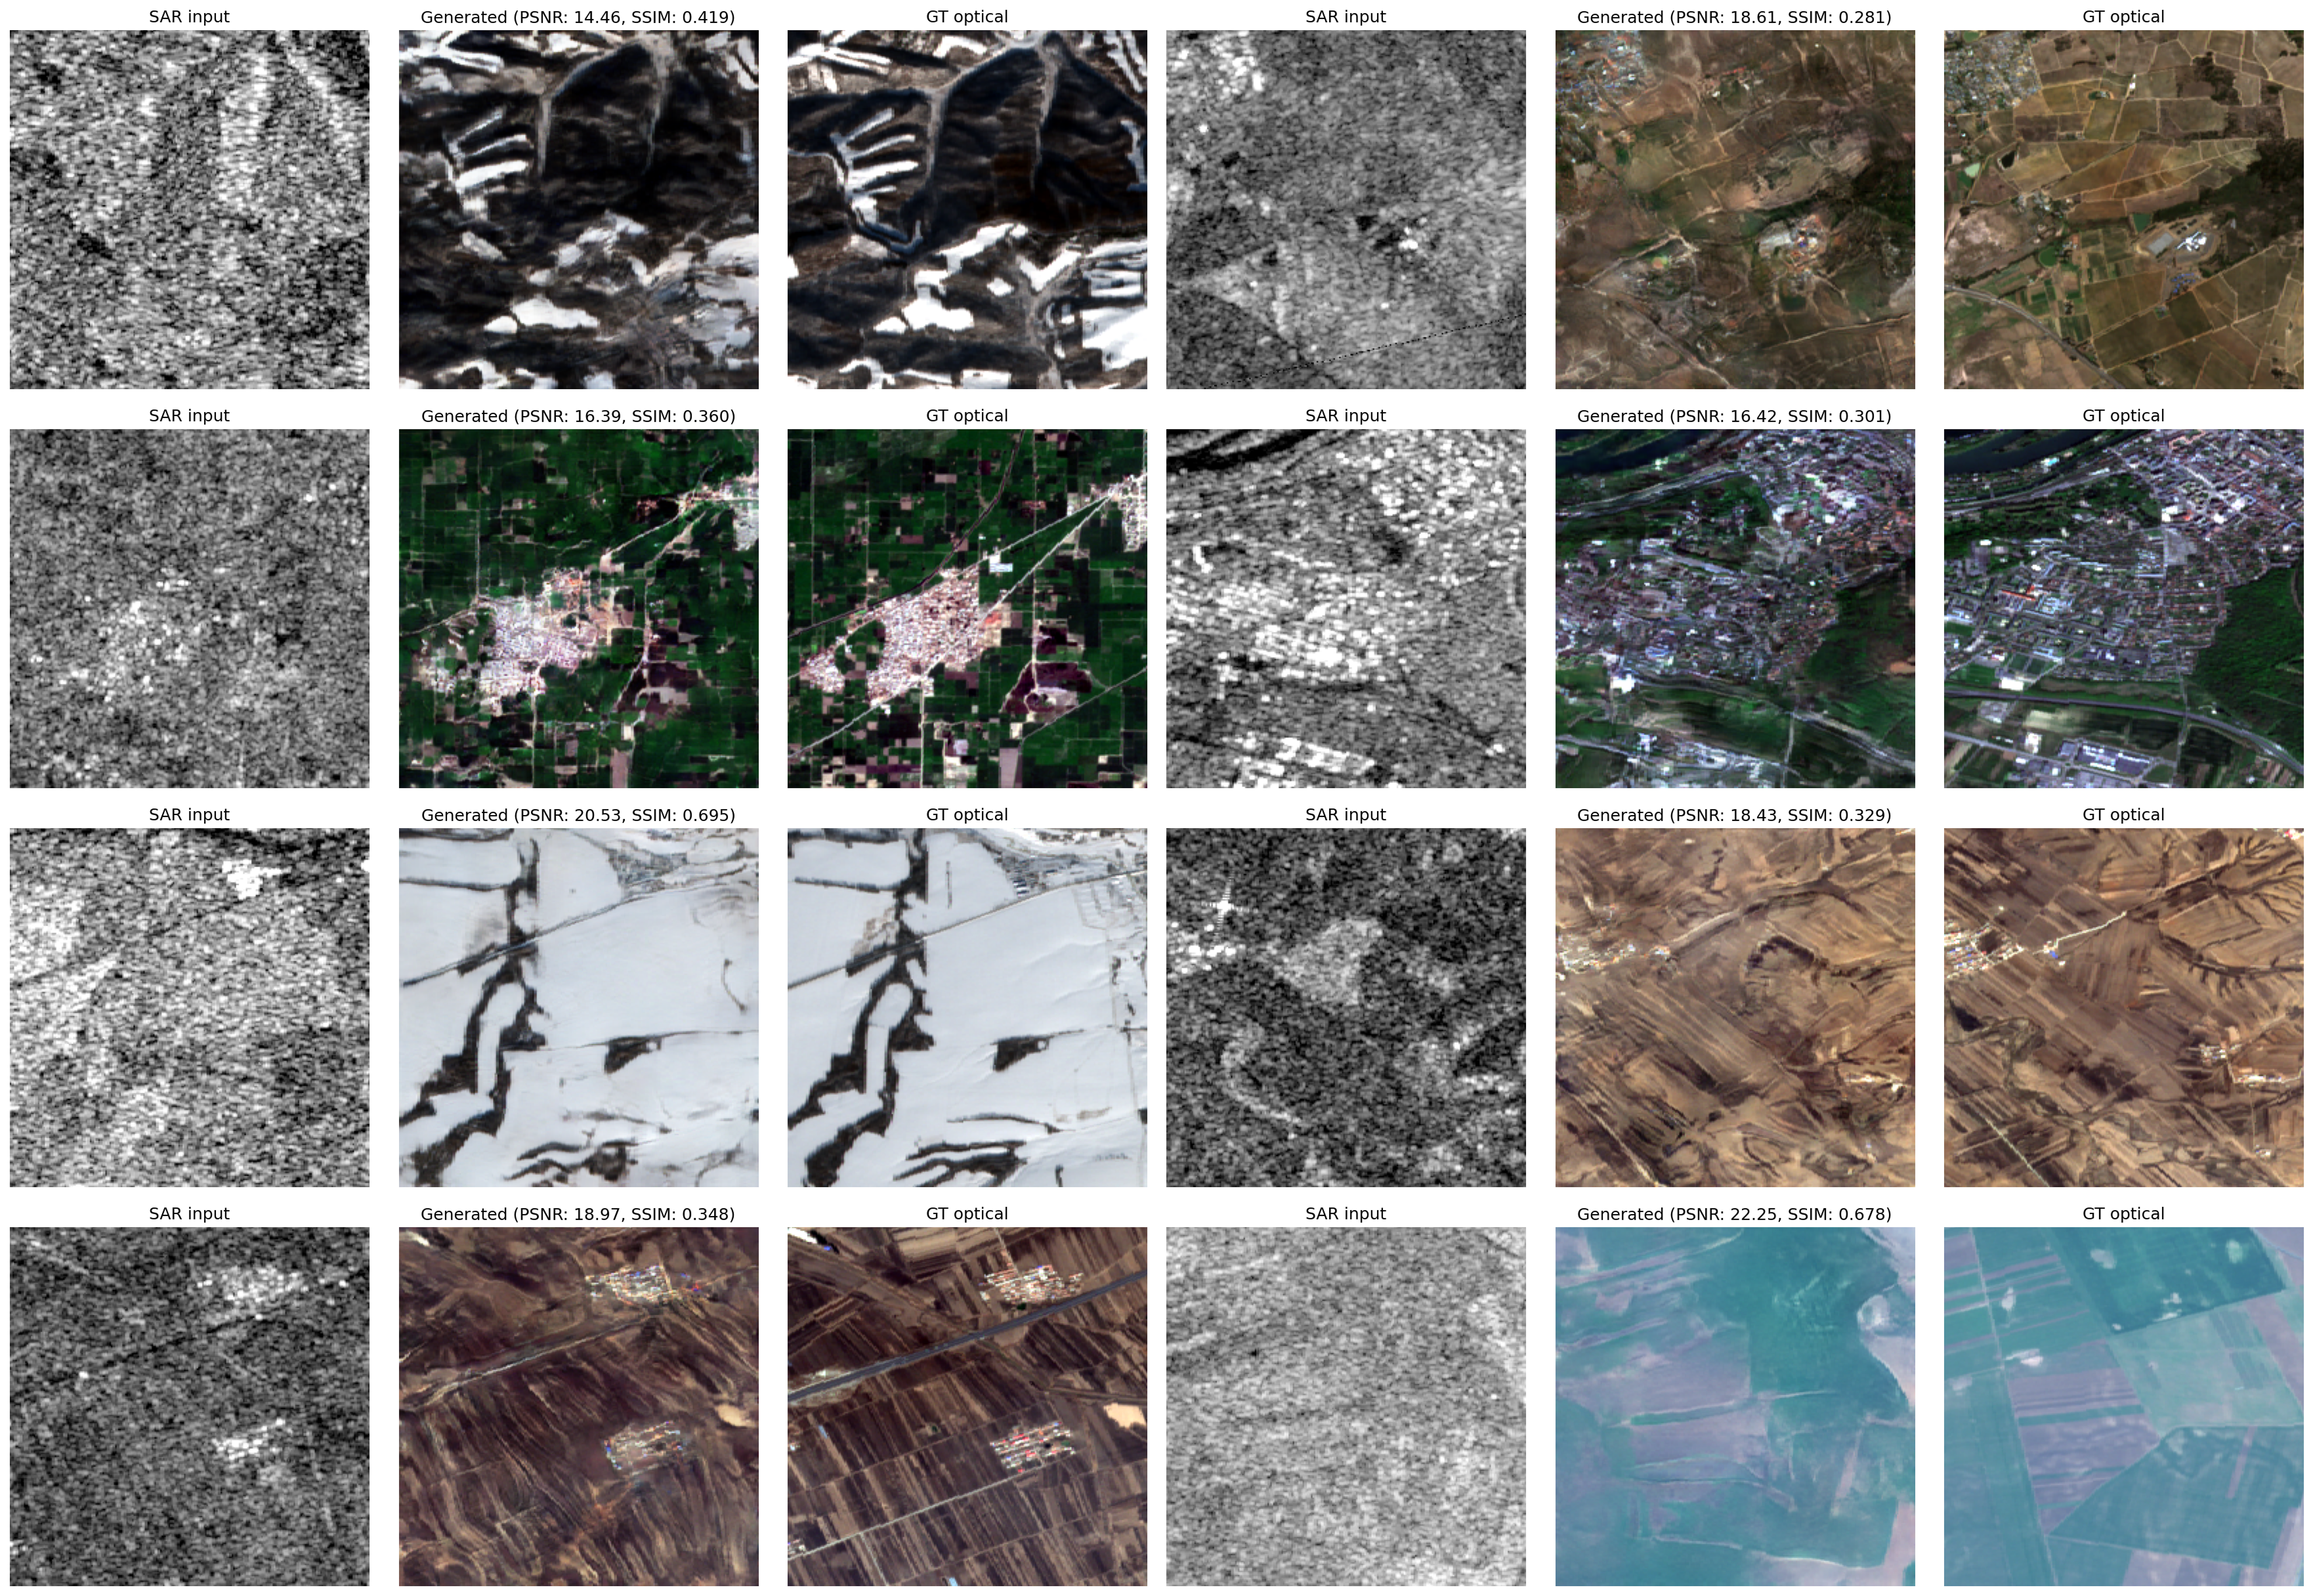
\includegraphics[width=\linewidth]{./images/convnextv2/output/val/huggingface_val_all.png}
    \caption{Результат обучения модели на базе ConvNeXtV2 на валидационной выборке. Столбцы слева направо: (а) входное SAR-изображение; (б) сгенерированное изображение; (в) целевое оптическое изображение (ground truth).}
    \label{fig:huggingface_val_all}
\end{figure}

Результаты обучения модели на базе ConvNeXtV2 показаны на рисунке~\ref{fig:huggingface_val_all}. Структуры и текстура восстанавливаются отлично, однако проступают семантические галлюцинации: на нижнем правом изображении модель не воспроизвела дорогу и чёткие границы полей, подставив естественные, но не отвечающие реальной сцене объекты. Это след всё того же доменного разрыва и ограниченной способности предобученного бэкбона моделировать радиометрическую вариативность SAR-изображений~--- основной трудности кросс-модального перевода при дефиците данных и вычислительных ресурсов.
\paragraph{Анализ количественных показателей}
На полной валидационной выборке (2263 пары, 5 сцен) модель даёт $\text{PSNR} = 17.95\,\text{dB}$, $\text{SSIM} = 0.404$, $\text{LPIPS} = 0.300$, $\text{FID} = 93.5$. Картина типична для ill-posed кросс-модального перевода: PSNR и SSIM заметно выше, чем у базовых Pix2Pix и CycleGAN, а FID остаётся высоким. Каскадный декодер с билинейным upsampling и групповой нормализацией сглаживает высокочастотные осцилляции; математически такое сглаживание поднимает pixel-level метрики (PSNR, SSIM), но визуально оборачивается умеренной спектральной размытостью на границах сложных текстур. Связанный с этим высокий FID фиксирует статистическое рассогласование распределений сгенерированной оптики и целевого домена~--- прямое следствие разрыва ImageNet$\leftrightarrow$SAR и того же ограничения бэкбона. Значение LPIPS ($0.300$) при этом остаётся конкурентным, то есть перцептивная согласованность и структурная целостность сцены сохраняются даже при просевшей частотной детализации.

Предложенная архитектура~--- осознанный инженерный компромисс. Отказ от избыточной ёмкости ради вычислительной эффективности и стабильного обучения дал высокие структурные метрики и ускорил инференс в разы относительно тяжёлых многоветвевых аналогов. Такой баланс оправдывает легковесную иерархическую схему там, где в приоритете скорость обработки, низкое энергопотребление или надёжное развёртывание на скромном железе, а макроструктурная корректность трансляции при этом сохраняется.

% ======================================================================
\subsection{LLW-Former: вейвлет-обусловленная архитектура с многокомпонентной функцией потерь}
\label{subsec:llwformer}

Легковесная модель из подраздела~\ref{subsec:lightweight_hierarchical_model}
(ConvNeXt~V2 с декодером в стиле U-Net) принята за \emph{базовую} архитектуру и
нулевую точку отсчёта для всего дальнейшего развития. Её анализ обнажил три
упирающихся в потолок качества ограничения.
Голова, предсказывающая RGB напрямую свёрткой $7{\times}7$, обучает
\emph{имплицитный} частотный базис и плохо разводит низкочастотный цвет и
высокочастотную текстуру, отчего границы систематически размываются.
Стандартный стем со страйдом~4 понижает разрешение обучаемым неинвертируемым
способом: частоты перемешиваются уже на входе, и функция потерь лишается рычага,
которым можно было бы избирательно регулировать вклад деталей.
Сюда добавляется и остаточная разрегистрация пар SAR\,/\,оптика в датасете SEN1-2
(медиана $\approx 1{,}2$~пикселя), постоянно тянущая пиксельные потери к
«безопасному» размытию.

Все три ограничения подводят к \emph{явной частотной декомпозиции}
входа и выхода и к функции потерь, устойчивой к мелким сдвигам. Этому и отвечает
разработанная архитектура \textbf{LLW-Former} (Learnable Lifting Wavelet
Former)\footnote{Архитектура создавалась итеративно; техническое имя реализации
в репозитории~--- \texttt{llwt}. Количественный вклад каждого компонента
оценивается обратной абляцией в главе~\ref{sec:results}, где строки таблицы
соответствуют последовательному отключению компонентов вплоть до базовой модели.}.
Далее приведена \emph{финальная} конфигурация модели целиком; промежуточные версии
не выносятся в изложение и фигурируют только как строки абляции.

\subsubsection*{Общий поток данных}

Генератор LLW-Former построен по схеме encoder--decoder со
skip-connections, в которой две позиции~--- стем и голова~--- заменены
вейвлет-блоками. Поток данных описывается цепочкой преобразований:
\begin{equation}
  \mathbf{x}_{\text{SAR}}
  \xrightarrow{\text{SARAdapter}}
  \mathbf{x}_{3}
  \xrightarrow{\text{HaarStem}}
  \mathbf{f}_{0}
  \xrightarrow{\text{ConvNeXt V2}}
  \{\mathbf{f}_{s_{0}},\,\mathbf{f}_{s_{1}},\,\mathbf{f}_{s_{2}},\,\mathbf{f}_{s_{3}}\}
  \xrightarrow{\text{Decoder}}
  \mathbf{S}
  \xrightarrow{\text{IHaar}}
  \mathbf{z}
  \xrightarrow{\tanh}
  \hat{\mathbf{y}}.
  \label{eq:flow}
\end{equation}
Здесь $\mathbf{x}_{\text{SAR}}\in\mathbb{R}^{1\times H\times W}$~---
одноканальный SAR-вход, $\mathbf{x}_{3}\in\mathbb{R}^{3\times H\times W}$~---
расширенное физически-осмысленное представление, $\mathbf{f}_{s_{i}}$~---
карты признаков $i$-й стадии бэкбона, $\mathbf{S}\in\mathbb{R}^{3\times 4
\times H/2\times W/2}$~--- тензор предсказанных Хаар-поддиапазонов,
$\mathbf{z}\in\mathbb{R}^{3\times H\times W}$~--- предтанжентные логиты,
$\hat{\mathbf{y}}\in[-1,1]^{3\times H\times W}$~--- финальный выход. Полная
блок-схема генератора приведена на рисунке~\ref{fig:arch}.

\begin{figure}[H]
  \centering
  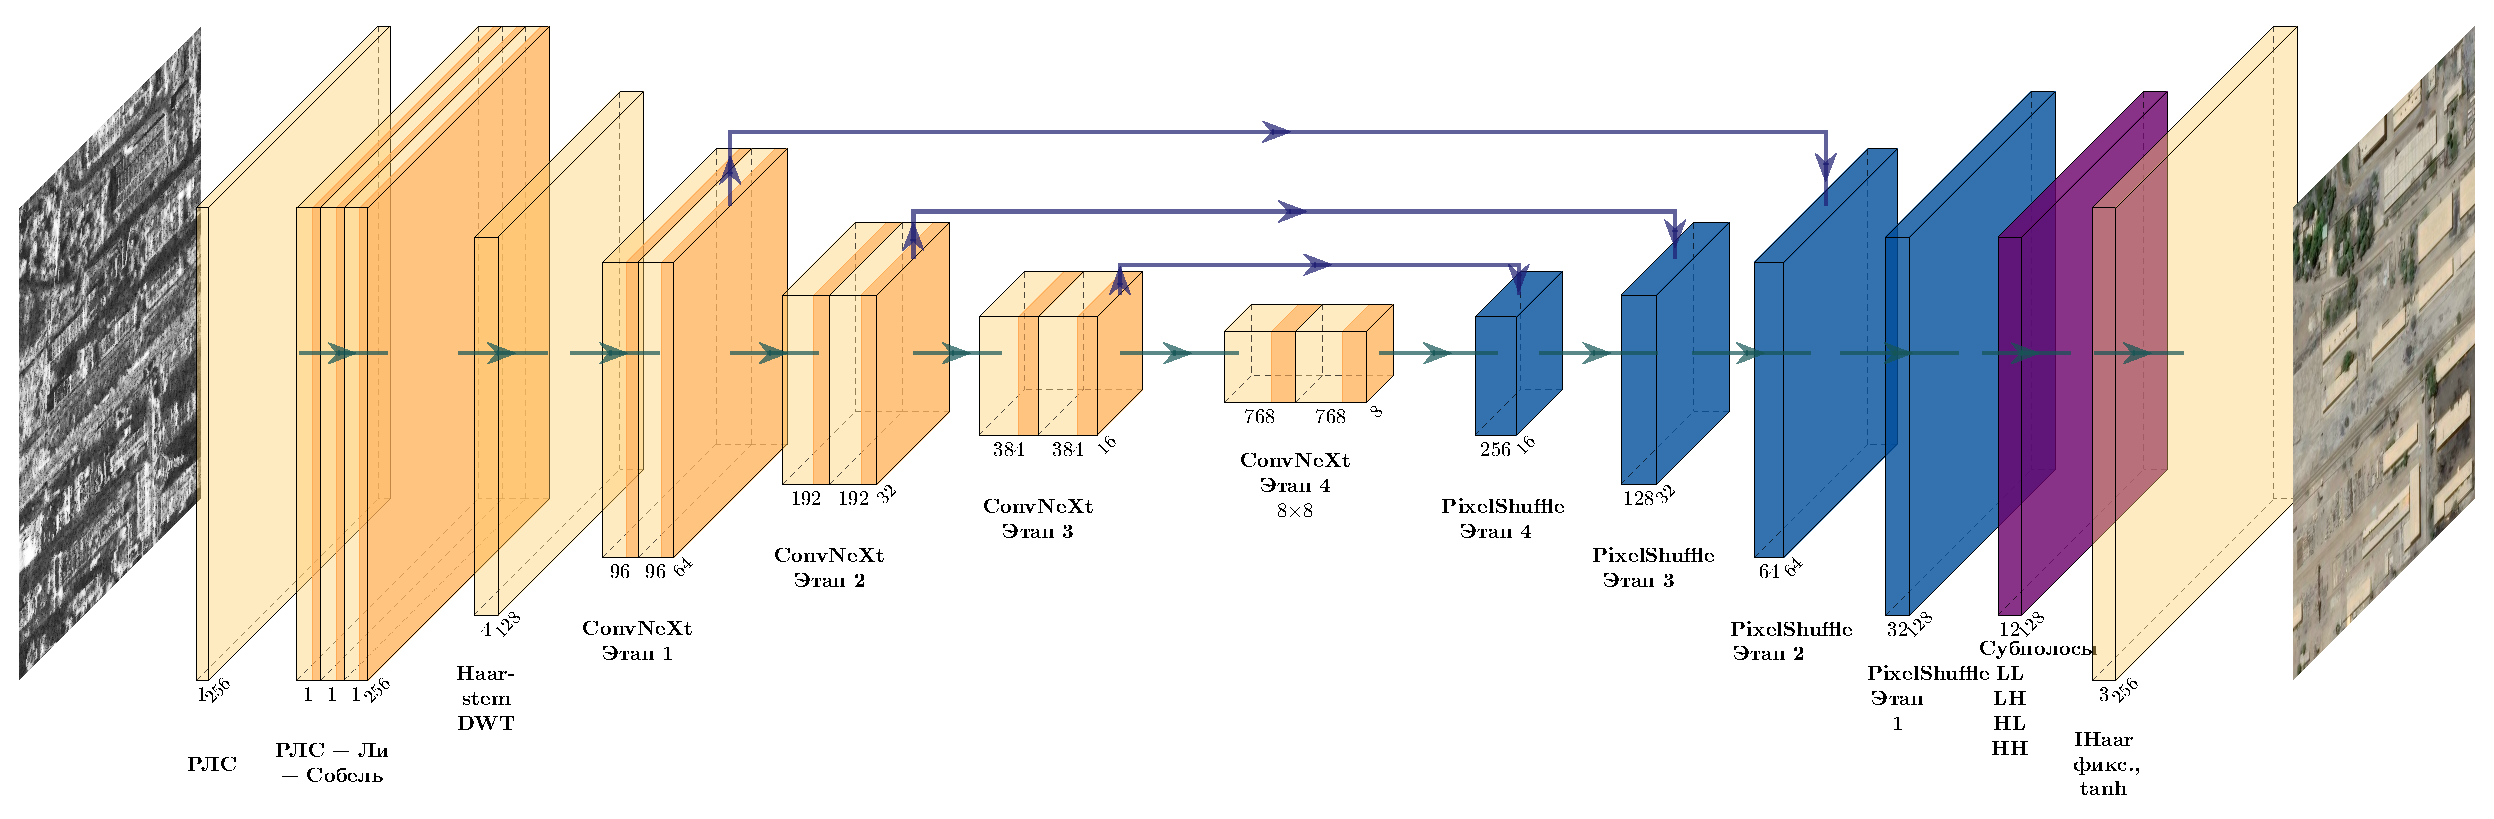
\includegraphics[width=\linewidth]{./images/llwt/llwt_v45.pdf}
  \caption{Архитектура генератора LLW-Former. SAR-вход проходит через адаптер
           физических каналов (РЛС\,+\,Ли\,+\,Собель), Хаар-стем заменяет
           стандартный patch-embed ConvNeXt~V2, четыре стадии бэкбона извлекают
           иерархические признаки, декодер с PixelShuffle и skip-соединениями
           восстанавливает разрешение, а обратное вейвлет-преобразование (IHaar)
           из предсказанных поддиапазонов LL/LH/HL/HH формирует полноразмерное
           RGB-изображение}
  \label{fig:arch}
\end{figure}

\subsubsection*{Адаптер SAR-входа}

SAR-сигнал по природе мультипликативен (спекл-шум логнормален), а оптика
аддитивна. Подавать исходную амплитуду прямо в свёрточную сеть невыгодно:
дисперсия каналов неоднородна, динамический диапазон растянут. Адаптер собирает
три канала~--- исходную амплитуду в $[-1,1]$, физически-мотивированный канал
(логарифм либо адаптивная фильтрация Ли в логарифмической области) и модуль
градиента Собеля. В финальной конфигурации вторым каналом взят фильтр Ли в
логарифмической области: по итогам внутренней абляции он оказался наиболее
выгодным для перцептивных метрик. Сеть получает на одну и ту же SAR-сцену
единичный, логарифмический и дифференциальный взгляд, и предобученному бэкбону
проще извлекать признаки.

\subsubsection*{Хаар-стем}

Стандартный стем ConvNeXt~V2~--- свёртка $4{\times}4$ со страйдом~4: понижение
разрешения в четыре раза обучаемым неинвертируемым способом. В предлагаемой модели
он заменён двухуровневым ортонормированным дискретным преобразованием Хаара.
Первый уровень разлагает $\mathbf{x}_{3}\in\mathbb{R}^{3\times H\times W}$ на
четыре поддиапазона размера $H/2\times W/2$; второй уровень применяется к
низкочастотной компоненте LL$_{1}$, давая ещё четыре поддиапазона размера
$H/4\times W/4$; высокочастотные поддиапазоны первого уровня пробрасываются вниз
с усреднением. Получается 21~канал на разрешении $H/4\times W/4$
(12~каналов от второго уровня и 9~уменьшённых от первого); их проецирует
$1{\times}1$-свёртка в размерность бэкбона (96 для Tiny, 128 для Base), после чего
следует LayerNorm. Выигрыш от такой замены двоякий. Понижение разрешения
становится \emph{интерпретируемым}: каждый канал лежит в фиксированном
вейвлет-базисе, и заранее ясно, какую частотную информацию он несёт. Вдобавок
низкие и высокие частоты разнесены по каналам явно, что согласуется со
статистикой естественных изображений и упрощает построение функции потерь.

\subsubsection*{Бэкбон ConvNeXt~V2}

Основной экстрактор признаков~--- предобученный ConvNeXt~V2~\cite{woo2023convnext}, где идеи
трансформеров (LayerNorm, GELU, depthwise-свёртки $7{\times}7$) сведены с чисто
свёрточной базой~\cite{liu2022convnet}. Во второй версии добавлен блок Global Response Normalization
(GRN), снижающий межканальную коллинеарность активаций, а обучение шло через
маскированное автоэнкодирование (FCMAE); для трансляции при
дефиците парных данных это ценное свойство. Структура блока ConvNeXt~V2 приведена на
рисунке~\ref{fig:cnxblock}. В разработанной модели используются две конфигурации
бэкбона: \texttt{convnextv2-tiny-22k-224} и \texttt{convnextv2-base-22k-224}
(сопоставление~--- в таблице~\ref{tab:backbones}); стем заменяется собственным
Хаар-стемом, четыре остальные стадии используются без изменений и инициализируются
предобученными весами.

\begin{figure}[H]
  \centering
  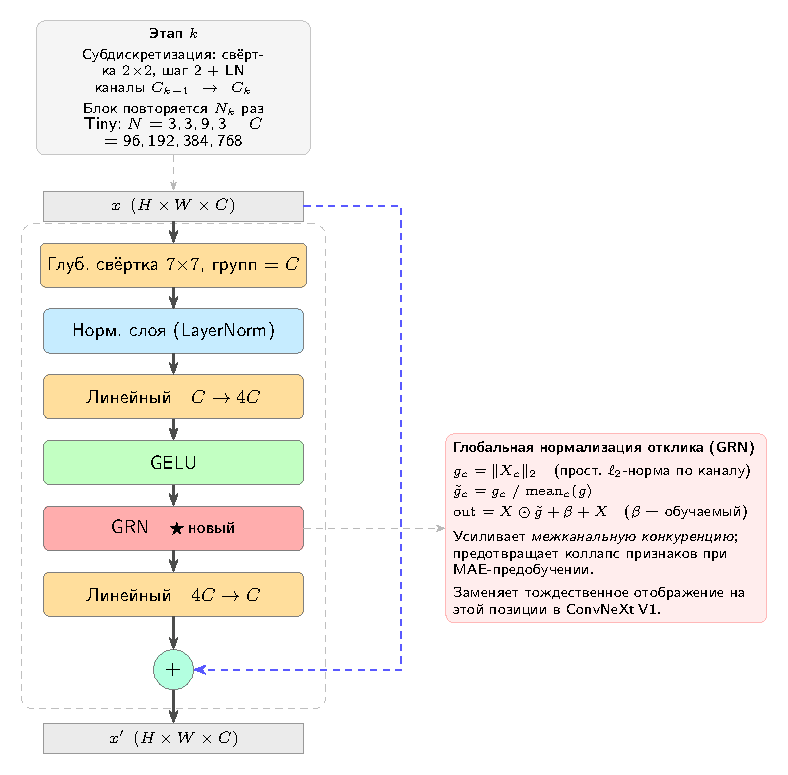
\includegraphics[width=0.42\linewidth]{./images/convnextv2/convnextv2_block.pdf}
  \caption{Строительный блок ConvNeXt~V2: depthwise-свёртка $7{\times}7$,
           LayerNorm, расширяющая $1{\times}1$-свёртка, GELU, блок Global Response
           Normalization (GRN) и сужающая $1{\times}1$-свёртка с остаточной связью}
  \label{fig:cnxblock}
\end{figure}

\begin{table}[H]
  \caption{Сопоставление конфигураций бэкбона ConvNeXt~V2}
  \label{tab:backbones}
  \centering
  \begin{tabular}{lcc}
    \toprule
    Характеристика & Tiny & Base \\
    \midrule
    Бэкбон Hugging Face & convnextv2-tiny-22k-224 & convnextv2-base-22k-224 \\
    Каналы стадий ($d_{0}{\dots}d_{3}$) & 96/192/384/768 & 128/256/512/1024 \\
    Параметры генератора & $\approx$\,29\,M & $\approx$\,88\,M \\
    Размер обучающего батча & 8 & 6 \\
    Среднее время эпохи & $\approx$\,260~с & $\approx$\,470~с \\
    Видеопамять (BF16) & $\approx$\,15.5~ГБ & $\approx$\,18.5~ГБ \\
    \bottomrule
  \end{tabular}
\end{table}

\subsubsection*{Декодер с PixelShuffle}

Декодер построен из четырёх последовательных блоков, каждый из которых удваивает
пространственное разрешение операцией PixelShuffle (рисунок~\ref{fig:pixelshuffle}).
Блок (рисунок~\ref{fig:decblock}) состоит из проекции $1{\times}1$, перестановки
каналов в пространство (PixelShuffle), конкатенации со skip-признаками
соответствующего уровня энкодера по схеме U-Net и двухступенчатой свёрточной
обработки $3{\times}3$ с групповой нормализацией, активацией GELU и остаточной
связью. Терминальный блок выдаёт карту размерности $(B,\,32,\,H/2,\,W/2)$, на
которой строится поддиапазонная голова. Числа каналов в блоках зависят от ёмкости
бэкбона: для Tiny это $768{\to}256{\to}128{\to}64{\to}32$, для Base~---
$1024{\to}256{\to}128{\to}64{\to}32$.

\begin{figure}[H]
  \centering
  \begin{minipage}[t]{0.46\linewidth}
    \centering
    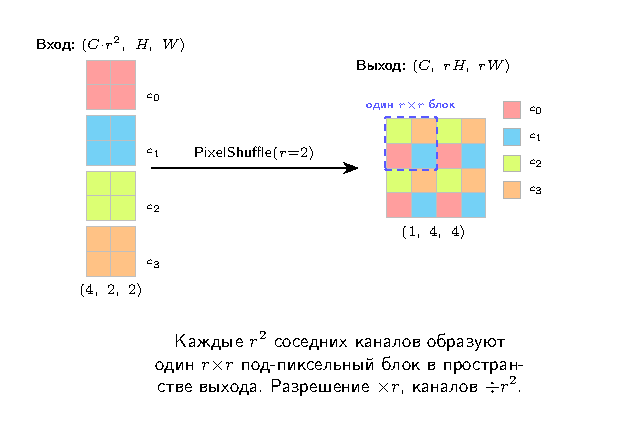
\includegraphics[width=\linewidth]{./images/llwt/pixelshuffle.pdf}
    \caption{Операция PixelShuffle: перенос каналов в пространственное разрешение
             (повышение разрешения $\times 2$ без обучаемой деконволюции,
             свободное от «шахматных» артефактов)}
    \label{fig:pixelshuffle}
  \end{minipage}\hfill
  \begin{minipage}[t]{0.46\linewidth}
    \centering
    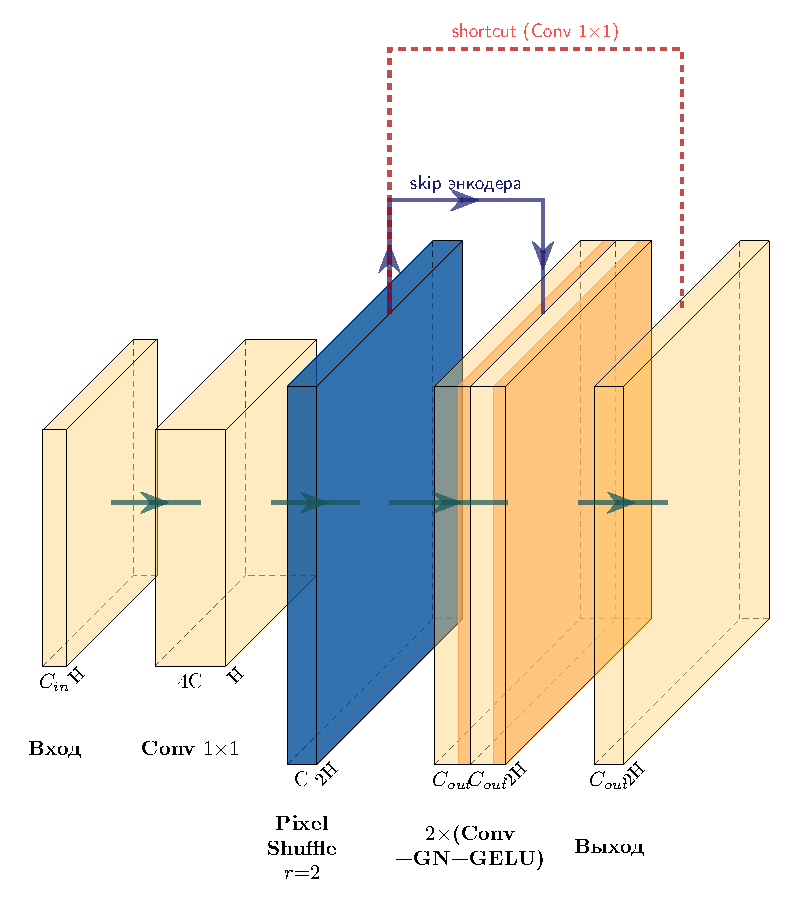
\includegraphics[width=\linewidth]{./images/llwt/decoder_block.pdf}
    \caption{Блок декодера \texttt{ConvUpsampleBlock}: $1{\times}1$-проекция,
             PixelShuffle, конкатенация со skip-признаками и две свёртки
             $3{\times}3$ (GroupNorm, GELU) с остаточной связью}
    \label{fig:decblock}
  \end{minipage}
\end{figure}

\subsubsection*{Голова с обратным Хаар-преобразованием}

Принципиальная особенность модели~--- \emph{явное предсказание
поддиапазонов Хаара} вместо RGB. Терминальная карта декодера
$(B,\,32,\,H/2,\,W/2)$ пропускается через свёртку $7{\times}7$ с отражённым
padding, выдающую 12 каналов на том же разрешении. Эти 12 каналов интерпретируются
как тензор $\mathbf{S}=(\mathbf{LL},\mathbf{LH},\mathbf{HL},\mathbf{HH})$ из четырёх
поддиапазонов по три RGB-канала. Затем применяется фиксированное обратное
Хаар-преобразование:
\begin{equation}
  \mathbf{z}=\mathrm{IHaar}(\mathbf{S})
            =\mathrm{PixelShuffle}_{2}\bigl(\mathbf{W}^{\top}\!\cdot\mathbf{S}\bigr),
  \label{eq:ihaar}
\end{equation}
где $\mathbf{W}$~--- ортонормированная Хаар-матрица $4{\times}4$; финальный выход
$\hat{\mathbf{y}}=\tanh(\mathbf{z})$. У такой головы есть несколько полезных
свойств. Обратное преобразование точно инверсно прямому ($\mathbf{W}^{\top}
=\mathbf{W}^{-1}$): на эталонных поддиапазонах вход и выход совпадают с точностью
до машинного нуля, что подтверждено модульными тестами. Нулевая инициализация
свёртки $7{\times}7$ на нулевой итерации даёт тождественно нулевые поддиапазоны, а
после $\tanh$~--- серое изображение; такой безопасный warm-start лишает
дискриминатор лёгкой победы на первых десятках шагов. Наконец, любая потеря,
наложенная прямо на $\mathbf{S}$, действует в заранее известном частотном базисе.

\subsubsection*{Дискриминатор}

Дискриминатор реализован как условный многомасштабный PatchGAN
(рисунок~\ref{fig:dis}, верхняя ветвь): на вход подаётся конкатенация
$[\mathbf{x}_{\text{SAR}},\mathbf{y}]\in\mathbb{R}^{4\times H\times W}$, пять
свёрточных слоёв с LeakyReLU формируют две карты логитов на разных рецептивных
полях ($70{\times}70$ и $46{\times}46$), что одновременно контролирует крупную
структуру и локальную текстуру. Помимо логитов, дискриминатор возвращает
промежуточные активации каждого слоя; они идут в потерю согласования
признаков (Feature Matching). В основной ветви спектральная нормализация
\emph{не} применяется: в сочетании с большим весом FM ($\lambda_{\text{fm}}=10$)
она лишает дискриминатор различающей способности (целью FM служит сам пул
признаков $D$). Поэтому взят рецепт pix2pixHD~--- многомасштабный
дискриминатор с FM и без спектральной нормализации. \emph{Нижняя} ветвь
рисунка~\ref{fig:dis}~--- высокочастотный дискриминатор HF-D, действующий на
высокочастотном остатке оптики и стабилизируемый спектральной нормализацией;
он составляет ключевой элемент новизны и подробно рассмотрен в
подразделе~\ref{subsec:hfd}.

\begin{figure}[H]
  \centering
  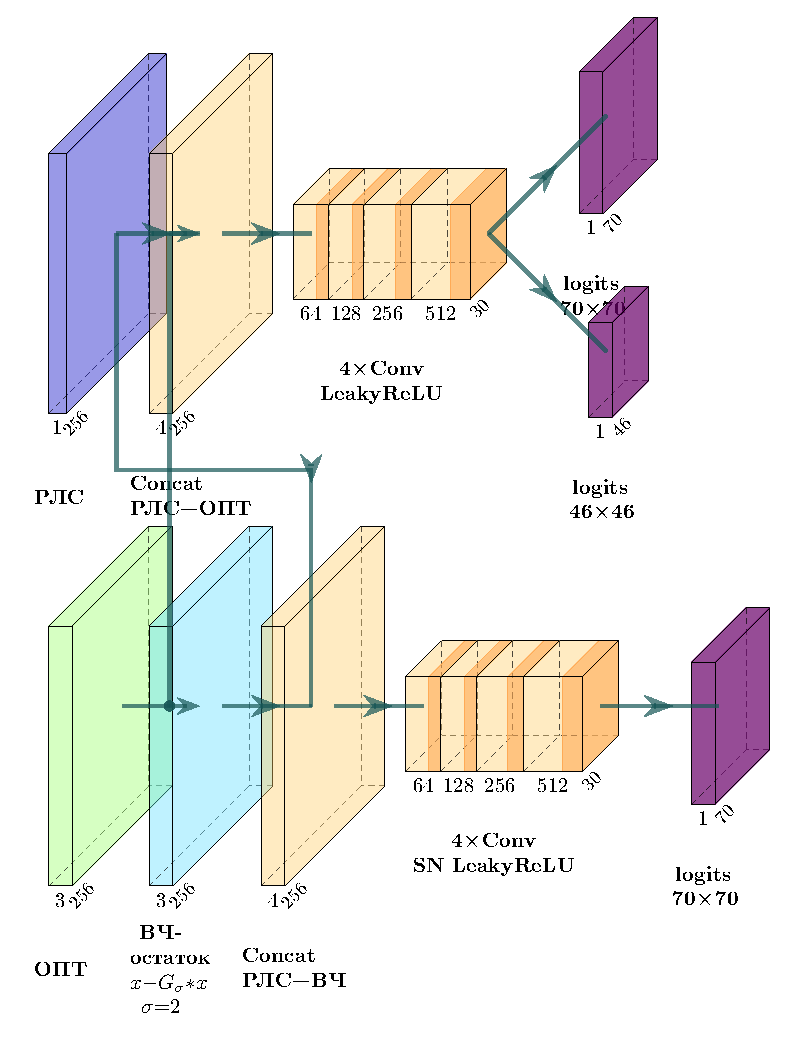
\includegraphics[width=0.62\linewidth]{./images/llwt/discriminator.pdf}
  \caption{Дискриминаторная схема LLW-Former. \emph{Верхняя ветвь}~--- основной
           условный многомасштабный PatchGAN на паре $[\text{РЛС},\text{оптика}]$ с
           двумя картами логитов ($70{\times}70$ и $46{\times}46$), без спектральной
           нормализации (рецепт pix2pixHD). \emph{Нижняя ветвь}~--- высокочастотный
           дискриминатор HF-D: вход $[\text{РЛС},\,h(\text{оптика})]$, где
           $h(x)=x-G_\sigma{*}x$ ($\sigma=2$)~--- высокочастотный остаток, со
           спектральной нормализацией на каждом слое (см.~\ref{subsec:hfd})}
  \label{fig:dis}
\end{figure}

\subsubsection*{Функция обучения}

Полная функция потерь генератора имеет вид:
\begin{equation}
  \mathcal{L}_{G} = \lambda_{\text{gan}}\,\mathcal{L}_{\text{gan}}
                  + \lambda_{\text{fm}}\,\mathcal{L}_{\text{fm}}
                  + \lambda_{\text{msssim}}\,\mathcal{L}_{\text{msssim}}
                  + \lambda_{\text{lpips}}\,\mathcal{L}_{\text{lpips}}
                  + \lambda_{\text{ffl}}\,\mathcal{L}_{\text{ffl}}
                  + \lambda_{\text{pb}}\,\mathcal{L}_{\text{pb}}
                  + \lambda_{\text{nce}}\,\mathcal{L}_{\text{nce}}.
  \label{eq:total}
\end{equation}
Веса и назначение слагаемых сведены в таблице~\ref{tab:lossw}; каждая
компонента отвечает за конкретный класс артефактов.

\begin{table}[H]
  \caption{Веса слагаемых функции потерь генератора в финальной конфигурации}
  \label{tab:lossw}
  \centering
  \begin{tabular}{lcl}
    \toprule
    Слагаемое & Вес $\lambda$ & Назначение \\
    \midrule
    $\mathcal{L}_{\text{gan}}$ (LSGAN)               & 1.0  & состязательная компонента \\
    $\mathcal{L}_{\text{fm}}$  (Feature Matching)    & 10.0 & стабилизация GAN \\
    $\mathcal{L}_{\text{msssim}}$                    & 1.0  & структурная сохранность \\
    $\mathcal{L}_{\text{lpips}}$  (AlexNet)          & 2.0  & перцептивное соответствие \\
    $\mathcal{L}_{\text{ffl}}$ (Focal Frequency)     & 10.0 & резкость в спектре Фурье \\
    $\mathcal{L}_{\text{pb}}$ (per-band Haar $L_{1}$)& 2.0  & пиксельный канал в Хаар-базисе \\
    $\mathcal{L}_{\text{nce}}$ (PatchNCE)            & 0.1  & устойчивость к разрегистрации \\
    \bottomrule
  \end{tabular}
\end{table}

\paragraph{Состязательная потеря и согласование признаков.}
Используется LSGAN-формулировка, дающая устойчивые градиенты при насыщении
дискриминатора:
\begin{equation}
  \mathcal{L}_{\text{gan}}^{G} = \mathbb{E}_{\mathbf{x},\mathbf{y}}
     \bigl[(D(\mathbf{x},\hat{\mathbf{y}})-1)^{2}\bigr],\qquad
  \mathcal{L}_{\text{gan}}^{D}
   = \tfrac{1}{2}\mathbb{E}\bigl[(D(\mathbf{x},\mathbf{y})-1)^{2}\bigr]
   + \tfrac{1}{2}\mathbb{E}\bigl[D(\mathbf{x},\hat{\mathbf{y}})^{2}\bigr].
\end{equation}
Feature Matching~--- среднее $L_{1}$-расстояние между промежуточными активациями
дискриминатора для эталонной и сгенерированной пар:
\begin{equation}
  \mathcal{L}_{\text{fm}} = \frac{1}{L}\sum_{l=1}^{L}
     \bigl\|D^{(l)}(\mathbf{x},\mathbf{y})-D^{(l)}(\mathbf{x},\hat{\mathbf{y}})\bigr\|_{1}.
\end{equation}
Высокий вес $\lambda_{\text{fm}}=10$ подобран эмпирически: его понижение до единицы
в промежуточной конфигурации роняло PSNR более чем на 1~дБ за первые
50~эпох.

\paragraph{Структурная потеря MS-SSIM.}
Multi-scale SSIM~\cite{wang2003msssim} штрафует размытие на нескольких масштабах:
$\mathcal{L}_{\text{msssim}} = 1 - \mathrm{MS\text{-}SSIM}(\hat{\mathbf{y}},\mathbf{y})$.
В отличие от $L_{1}$, MS-SSIM не наказывает локальные сдвиги яркости, но требует
сохранения структурных корреляций, что критично для городских и прибрежных сцен.

\paragraph{Перцептивная потеря LPIPS.}
Перцептивная потеря~\cite{zhang2018unreasonable}~--- взвешенное расстояние между
признаками замороженной сети AlexNet:
\begin{equation}
  \mathcal{L}_{\text{lpips}}=\sum_{l}\frac{1}{H_{l}W_{l}}
     \sum_{h,w}\bigl\|w_{l}\odot
     (\phi_{l}(\hat{\mathbf{y}})_{h,w}-\phi_{l}(\mathbf{y})_{h,w})\bigr\|_{2}^{2}.
\end{equation}

\paragraph{Focal Frequency Loss.}
FFL~\cite{jiang2021ffl} штрафует расхождение в спектре Фурье с фокусной
нелинейностью, акцентирующей плохо предсказанные частоты:
\begin{equation}
  \mathcal{L}_{\text{ffl}}=\frac{1}{HW}\sum_{u,v}
    w(u,v)\,|F_{\hat{\mathbf{y}}}(u,v)-F_{\mathbf{y}}(u,v)|^{2},\qquad
  w(u,v)=|F_{\hat{\mathbf{y}}}-F_{\mathbf{y}}|^{\alpha},\ \alpha=1.
\end{equation}
FFL действует в глобальном спектре, а поддиапазонная Хаар-потеря~--- в
локальных поддиапазонах, и две эти потери дополняют друг друга.

\paragraph{Поддиапазонная Хаар-потеря.}
Поскольку голова выдаёт поддиапазоны $\mathbf{S}_{\text{pred}}$ напрямую,
естественно сопоставлять их с поддиапазонами эталона
$\mathbf{S}_{\text{gt}}=\mathrm{HaarDown}(\mathbf{y})$ покомпонентно:
\begin{equation}
  \mathcal{L}_{\text{pb}}=\frac{\sum_{b}w_{b}\bigl\|
                              \mathbf{S}_{\text{pred}}^{(b)}-
                              \mathbf{S}_{\text{gt}}^{(b)}\bigr\|_{1}}
                              {\sum_{b}w_{b}},\quad
  b\in\{\text{LL},\text{LH},\text{HL},\text{HH}\}.
\end{equation}
Вектор весов $w=(1.0,\,1.5,\,1.5,\,2.0)$ усиливает вклад поддиапазонов деталей;
знаменатель нормирует сумму весов, и единственным управляющим параметром остаётся
$\lambda_{\text{pb}}$. К произвольной архитектуре такая потеря \emph{неприменима}:
ей нужно, чтобы выход модели был покомпонентно интерпретируем в Хаар-базисе,~---
а это как раз и обеспечивает голова с обратным Хаар-преобразованием.

\paragraph{Контрастная потеря PatchNCE.}
Остаточная разрегистрация пар SAR\,/\,оптика давит любую попиксельную потерю в
сторону размытия. Чтобы градиент был согласован с \emph{содержанием}, а
не с точным положением пикселя, привлечён контрастный объектив
PatchNCE~\cite{park2020cut}. В отличие от исходной непарной формулировки,
здесь применяется \emph{позиционная} положительная выборка (положительная пара берётся в
той же координате), а энкодер генератора повторно используется как feature-сеть:
\begin{equation}
  \mathcal{L}_{\text{nce}}=\sum_{l\in\mathcal{L}}\frac{1}{N_{l}}\sum_{i}
    -\log\frac{\exp\bigl(\langle v_{i}^{l,\hat{y}},v_{i}^{l,y}\rangle/\tau\bigr)}
              {\sum_{j}\exp\bigl(\langle v_{i}^{l,\hat{y}},v_{j}^{l,y}\rangle/\tau\bigr)},
\end{equation}
где $v^{l,\cdot}$~--- нормированные эмбеддинги патчей на стадии $l$ бэкбона,
$\mathcal{L}=\{0,1,2,3\}$, $N_{l}=256$, $\tau=0{,}07$.

% ======================================================================
\subsection{Высокочастотный дискриминатор (HF-D)}
\label{subsec:hfd}

Несмотря на частотно-симметричную архитектуру и многокомпонентную функцию потерь,
выходы базовой модели остаются перцептивно мягкими. Профилирование (глава~\ref{sec:results},
раздел~\ref{sec:results:negative}) локализует дефицит в средне- и высокочастотном
диапазоне, а две естественные гипотезы его устранения~--- обучаемая регистрация пар и
инвариантная к сдвигу статистическая потеря~--- не подтвердились (там же).
Эти негативные результаты указывают на единственный работающий механизм: \emph{состязательное}
давление, прицельно направленное на высокие частоты. На этом и построен главный элемент
новизны настоящей работы~--- \textbf{высокочастотный дискриминатор} (high-frequency
discriminator, HF-D).

Пусть $h(x)=x-g_\sigma * x$~--- высокочастотный остаток изображения, где $g_\sigma$~---
гауссово ядро ($\sigma=2$). HF-D, обозначаемый $D_H$,~--- условный PatchGAN со
спектральной нормализацией на каждой свёртке, принимающий конкатенацию SAR-условия $s$
с высокочастотным остатком оптического изображения, $D_H([\,s,\;h(y)\,])$, и обучаемый
состязательно против выхода генератора $\hat{y}=G(s)$. В LSGAN-формулировке:
\begin{align}
  \mathcal{L}_{D_H} &= \tfrac{1}{2}\,\mathbb{E}\bigl[(D_H([s,h(y)])-1)^{2}\bigr]
                     + \tfrac{1}{2}\,\mathbb{E}\bigl[D_H([s,h(\hat{y})])^{2}\bigr],\\
  \mathcal{L}^{G}_{H} &= \mathbb{E}\bigl[(D_H([s,h(\hat{y})])-1)^{2}\bigr].
\end{align}
Слагаемое $\lambda_H\,\mathcal{L}^{G}_{H}$ ($\lambda_H=1$) добавляется к целевой функции
генератора~\eqref{eq:total} в дополнение к основному дискриминатору. HF-D
оценивает \emph{реалистичность деталей}, а не их попиксельное положение, поэтому он устойчив к
остаточной разрегистрации, губящей пиксельную супервизию, и при этом навязывает
когерентность, которой лишены статистические потери. Работа на высокочастотном остатке
концентрирует ёмкость дискриминатора именно на дефицитных средне-/высокочастотных
октавах.

Спектральная нормализация на каждой свёртке здесь критична: ранний поддиапазонный дискриминатор
без неё расходился (логиты порядка $10^5$). HF-D \emph{аддитивен} к основному условному
дискриминатору и независим от него; при $\lambda_H=0$ модель в точности сводится к
базовой, что даёт чистую абляцию по одному флагу. Важно и то, что HF-D работает
\emph{только на этапе обучения}: на инференсе генератор не меняется, и вычислительная
стоимость предсказания остаётся прежней. Экспериментальная проверка HF-D (отложенный A/B и
контролируемое сравнение) приведена в разделе~\ref{sec:results:hfd}.

\newpage